\documentclass[12pt]{article}
\usepackage[T1]{fontenc}
\usepackage{lmodern}  % 強制使用 Latin Modern
\usepackage{fontspec}
\usepackage{graphicx}  % 支援插入圖片
\usepackage{amsmath}

\usepackage[backend=biber, style=numeric, sorting=none]{biblatex}

\usepackage{csquotes}
\usepackage{tocloft}
\addbibresource{references.bib}  % 引入你的.bib文件


\renewcommand{\cftsecleader}{\cftdotfill{\cftdotsep}}  % 節
\renewcommand{\cftsubsecleader}{\cftdotfill{\cftdotsep}}  % 小節
\renewcommand{\cftsubsubsecleader}{\cftdotfill{\cftdotsep}}  % 子小節


% 英文字體
\newfontface\englishfont{Times New Roman}

\setmainfont[
    ItalicFont={Times New Roman Italic},
    BoldFont={Times New Roman Bold},
    BoldItalicFont={Times New Roman Bold Italic}
]{Times New Roman}


% 中文字體
\usepackage{xeCJK}
\setCJKmainfont{標楷體-繁}

\usepackage[top=2cm, bottom=2cm, left=2cm, right=2cm, a4paper]{geometry}

\usepackage{setspace}
\onehalfspacing 
\setlength{\parskip}{6pt}
\setlength{\parindent}{2em} 

\renewcommand{\contentsname}{\centering \LARGE \textbf{目錄}}

\begin{document}

\pagenumbering{roman}  
\setcounter{page}{1}  % 從 I 開始

%=================================================={{{中文摘要}}}==================================================
\section*{\centering 摘要}  % 只讓標題置中
\addcontentsline{toc}{section}{摘要}  % 手動加入摘要到目錄
%==============================摘要內容==============================


%==============================摘要內容==============================
\newpage  % 插入換頁命令,將目錄和後續內容分開
%=================================================={{{中文摘要}}}==================================================

%=================================================={{{英文摘要}}}==================================================
\section*{\centering Abstract}  % 只讓標題置中
\addcontentsline{toc}{section}{Abstract}  % 手動加入摘要到目錄
%==============================摘要內容==============================


%==============================摘要內容==============================
\newpage  % 插入換頁命令,將目錄和後續內容分開
%=================================================={{{英文摘要}}}==================================================

%=================================================={{{目錄}}}==================================================
\begin{center}
\tableofcontents  % 插入目錄,並置中
\thispagestyle{empty}  % 讓目錄頁沒有頁碼
\end{center}
\newpage  % 插入換頁命令,將目錄和後續內容分開
%=================================================={{{目錄}}}==================================================

%=================================================={{{內文}}}==================================================
\pagenumbering{arabic}  % 開始使用阿拉伯數字頁碼
\setcounter{page}{1}  % 設定頁碼從 1 開始

\section{緒論}
\section{文獻探討與回顧}
\section{研究方法及流程}
\section{研究結果}
\section{結論}
\subsection{子標題}  

\hspace{2em}你好世界, \englishfont{this is an example of mixed English and Chinese.}詞曰:

,如圖,話說天下大勢.分久必合,合久必分:周末七國分爭,并入於秦。及秦滅之後,楚、漢分爭,又并入於漢。漢朝自高祖斬白蛇而起義,一統天下。後來光武中興,傳至獻帝,遂分為三國。推其致亂之由,殆始於桓、靈二帝。桓帝禁錮善類,崇信宦官。及桓帝崩,靈帝即位,大將軍竇武、太傅陳蕃,共相輔佐。時有宦官曹節等弄權,竇武、陳蕃謀誅之,作事不密,反為所害。中涓自此愈橫。

建寧二年四月望日,帝御溫德殿。方陞座,殿角狂風驟起,只見一條大青蛇,從梁上飛將下來,蟠於椅上。帝驚倒,左右急救入宮,百官俱奔避。須臾,蛇不見了。忽然大雷大雨,加以冰雹,落到半夜方止,壞卻房屋無數。建寧四年二月,洛陽地震;又海水泛溢,沿海居民,盡被大浪捲入海中。光和元年,雌雞化雄。六月朔,黑氣十餘丈,飛入溫德殿中。秋七月,有虹見於玉堂;五原山岸,盡皆崩裂。種種不祥,非止一端。




\hspace{2em}群臣以災異之由,議郎蔡邕上疏,以為蜺

%==============================圖片==============================
\begin{figure}[h]
    \centering
    \renewcommand{\figurename}{圖} %顯示圖1,不是figureat1
    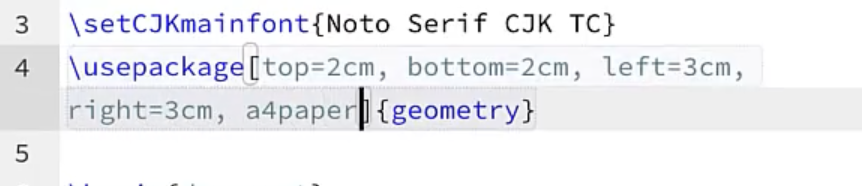
\includegraphics[width=0.5\textwidth]{截圖 2025-01-24 03.21.17.png}     %圖片檔案名稱
    \caption{這是圖片的標題}    %圖片檔案名稱
    \label{fig:example2}    %為圖片添加標籤
    %\ref{fig:example1}
\end{figure}
%==============================圖片==============================


%==============================數學公式==============================
\begin{align}
    a &= b + c \label{eq:1}
    \\
    d &= e - f \label{eq:2}
    %式(\ref{eq:2})
\end{align}
%==============================數學公式==============================


時鉅(\ref{eq:2})根據文獻\cite{einstein1905},光電\cite{latexcompanion}效\cite{鄭智銘2006分散式儲存架構下的遠距環境監測系統之建構}應...鹿郡有兄弟三人:一名張角,一名張寶,一名張梁。那張角本是個不第秀才。因入山採藥,遇一老人,碧眼童顏,手執藜杖,喚角至一洞中,以天書三卷授之,曰:「此名太平要術。汝得之,當代天宣化,普救世人;若萌異心,必獲惡報。」角拜問姓名。老人曰:「吾乃南華老仙也。」言訖,化陣清風而去。

%==============================表格==============================
\begin{table}[ht]
    \centering
    \begin{tabular}{|c|c|c|}
    \hline
    項目  & 數量 & 價格 \\
    \hline
    蘋果  & 10  & 30   \\
    香蕉  & 5   & 15   \\
    橙子  & 8   & 20   \\
    \hline
    \end{tabular}
    \caption{水果表格}
    \label{tab:fruits}
\end{table}
%==============================表格==============================

\section{參考文獻}
\vspace{-3.5em}  % 減少與上方內容的間距
\renewcommand{\refname}{}  % 去除 "References" 標題
\printbibliography  % 列出參考文獻
\end{document}
%=================================================={{{內文}}}==================================================

